%!TEX root = ../main.tex
%% Chapter 2 - Openstack


\chapter{OpenStack}

This section gives a detailed description of the \textit{OpenStack} technology in order to better understand how it works.


%%--------------- section
\section{Definition}
\textit{OpenStack} is an open source project licensed under the \textit{Apache License 2.0} and consists of several projects (or services), which allow creating cloud infrastructures.
In other words it is \textit{a cloud operating system that controls large pools of compute, storage, and networking resources throughout a data center, all managed through a dashboard that gives administrators control while empowering their users to provision resources through a web interface.
}\cite{osdef}
Thus, OpenStack provides an out of the box IaaS solution.

%Different projects (or services) offered by OpenStack can be installed separately on different machines, but they are working together.
OpenStack offers different services that can be distributed across different machines in various configurations.
A list of these projects is given in the Table \ref{table:openstack_services_list}.
Only the projects Nova, Keystone, Horizon, Glance and Cinder were used for the experiments and will be discussed in more details below.
Figure \ref{fig:openstack_services_arch} shows how each service interacts with other services in a typical OpenStack environment.

%%--------------- section
\section{Services}

In this section, the different services used for the experiments are discussed in details.

\begin{figure}[h]
	\centering
	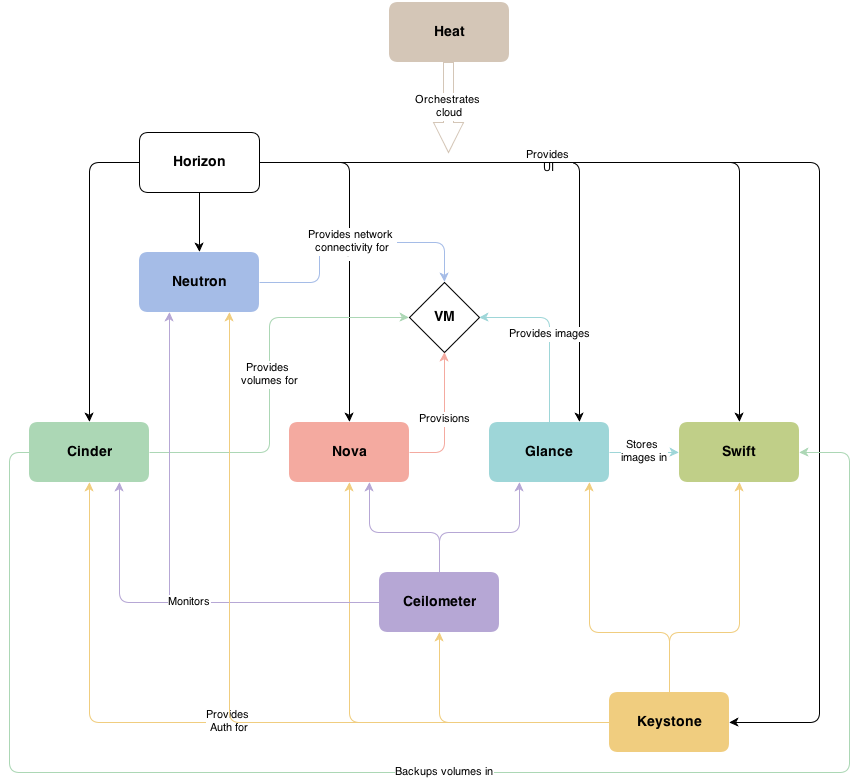
\includegraphics[scale=0.5]{figures/openstack_havana_conceptual_arch.png}
	\caption{Conceptual architecture of OpenStack Havana \cite{osarch}}
	\label{fig:openstack_services_arch}
\end{figure}

\begin{table}[h]
	\centering
	\begin{tabular}{|l|l|p{9.5cm}|}
		\hline
		\textbf{Project name} & \textbf{Service} & \textbf{Description}\\
		\hline
		Nova & Compute & Creates and manages virtual machines\\
		Keystone & Identity & Provides authentication and authorization\\
		Horizon & Dashboard & Web interface to manage all services\\
		Neutron & Networking & Manages networking for advanced network topologies\\
		Glance & Image & Provides a registry of virtual machine images\\
		Cinder & Block Storage & Provides persistent storage to VMs\\
		Swift & Object Storage & Stores data, including virtual images\\
		Ceilometer & Telemetry & Collects metering data (CPU and network costs)\\
		Heat & Orchestration & Deploys (complex) running cloud applications or stack (i.e. flavor, instance, network, etc.) described with templates (YAML text files)\\
		Trove & Database & Provides scalable and reliable cloud provisioning functionality for relational and non-relational database engines\\
		\hline
	\end{tabular}
	\caption{OpenStack services}
	\label{table:openstack_services_list}
\end{table}

\subsection{Nova}
Nova service is responsible for creating and managing virtual machines on demand.
Upon creating a virtual machine, the user can specify a flavor he wants to use.
The flavor allows to set the characteristics of a virtual machine: amount of RAM, number of virtual CPUs (VCPUs), sizes of root, ephemeral and swap disks.
By default, Nova provides some built-in set of flavors and the user can create more if needed.
Table \ref{table:flavors_list} shows characteristics of the built-in flavors (ephemeral and swap disks are set to 0).

\begin{table}[h]
	\centering
	\begin{tabular}{|l|l|l|l|}
		\hline
		\textbf{Flavor} & \textbf{\# of VCPUs} & \textbf{Disk size (GB)} & \textbf{RAM size (MB)}\\
		\hline
		m1.tiny & 1 & 1 & 512 \\
		m1.small & 1 & 20 & 2048 \\
		m1.medium & 2 & 40 & 4096 \\
		m1.large & 4 & 80 & 8192 \\
		m1.xlarge & 8 & 160 & 16384 \\
		\hline
	\end{tabular}
	\caption{Flavors}
	\label{table:flavors_list}
\end{table}


% OpenStack provides two different services to manage storage, namely \textit{Block Storage} and \textit{Object Storage}.
% As mentioned earlier, different OpenStack services can be installed separately, and there is no need to install all the services in order to have a virtual machine running.
% By default, when creating a virtual machine, it will have its own storage (i.e. a disk or a root disk), which is mandatory in order to install an operating system on it,
% and it does not need the Block Storage service. 
% However, Block Storage is required to extend the storage of a virtual machine in the future. 
% Coming back to flavors, ephemeral disk corresponds to the amount of disk space to use for the ephemeral partition when a virtual machine is launched. 
% These types of disks are bounded to the lifecycle of a virtual machine, meaning that if a virtual machine is terminated, all the data on the disk is lost. 
% However, the data persists after rebooting a virtual machine.\rp{These paragraphs are very complicated for reading, because there are many things you want to write about and they are important. Still try to first write everything about one storage and then continue to another one, without back and forward referencing. Something like Openstack has this and that, this is why one needs this, this is why we need that, these are the characteristics.}
% The root disk is a special case of ephemeral disk. 
% It is used to create a root partition (/) for a virtual machine and, unlike ephemeral disk, it is included in snapshots of the virtual machine. 
% If the size of the root disk is set to 0, this means that its size will be set to the one of image containing the operating system.
% Finally, there is also the possibility to add a swap disk to the virtual machine.
% The different storage solutions of OpenStack are summarized in Table \ref{table:storage_list}.

With these flavors, Nova already offers two ephemeral storage solutions for the virtual machines, namely the \textit{ephemeral disk} and the \textit{root disk}.
The ephemeral disk corresponds to the amount of disk space to use for the ephemeral partition when a virtual machine is launched. 
These types of disks are said ephemeral because they are bounded to the lifecycle of a virtual machine, meaning that if a virtual machine is terminated, all the data on the disk is lost. 
However, the data persists after rebooting a virtual machine.
This kind of ephemeral storage can be useful for storing temporarily a small amount of data in order to process them later.
The root disk is a special case of ephemeral disk. 
It is used to create a root partition on which the operating system will be installed.
Unlike the ephemeral disk, the root disk is included in snapshots of the virtual machine. 
By default, when creating a virtual machine, it will necessarily have a root disk that holds the operating system, and optionally an ephemeral disk to store temporary data which will not appear in virtual machine snapshots.
% and it does not need the Block Storage service. 



Nova is also able to handle networking via the \texttt{nova-network} service. 
As networking is very complex, OpenStack decided to split the Nova project in two parts: one project, Nova, will be exclusively responsible for virtual machines and another project, Neutron, will be exclusively responsible for networking. 
The latter offers more features such as the possibility to create routers.
This allows to create quite complex networks if needed.
Thus, the \texttt{nova-network} is planned to be removed from the Nova project, and Neutron will be used in its place.
For our experiment, it was sufficient to only use Nova to manage networking instead of Neutron.






\subsection{Glance}
Glance service is responsible for providing a registry of virtual machine images.
A virtual machine image contains an image of an operating system, which is used to launch virtual machines. 
The uploaded images are stored on the same system that hosts the Image Service, in the \texttt{/var/lib/glance/images/} directory by default.

\subsection{Cinder}
Cinder is responsible for providing persistent storage to virtual machines in contrast to ephemeral storage offered by Nova. 
This persistent storage is also called volume. 
Unlike ephemeral storage, all data that is on a volume persists when a virtual machine is terminated. 
This volume is similar to the \textit{Amazon Elastic Block Storage (Amazon EBS)}\footnote{\url{http://aws.amazon.com/ebs}} 
and can be compared to an external hard disk drive (HDD) that is plugged into a computer: we say that the volume is attached to an instance. 
In order for the attached volume to be usable, it has to be mounted and formatted. 
Afterwards, data can be stored on the volume. 
The attached volume can also be made bootable, and thus replace the Nova root disk.
It has to be noted that one volume can only be attached to one instance at a time, but one instance can have several volumes attached to it.
This type of storage is useful to store important data and/or a large amount of data.

The different OpenStack storage solutions are summarized in Table \ref{table:storage_list}. 
This table shows the Object Storage solution which was not used in our experiment. 
This solution can be compared to the \textit{Amazon Simple Storage Service (Amazon S3)}\footnote{\url{http://aws.amazon.com/s3}} which allows to easily store and retrieve data from anywhere on the Web.

\begin{table}[h]
	\centering
	\begin{tabular}{|m{2cm}|m{3.8cm}|m{3.8cm}|m{3.8cm}|}
		\hline
		 & 
		\textbf{Ephemeral \newline storage} & 
		\textbf{Block storage} & 
		\textbf{Object storage}\\
		\hline
		\textbf{Used to} & 
		Run operating system and scratch space & 
		Add additional persistent storage to a virtual machine (VM) & 
		Store data, including VM images \\
		\hline
		\textbf{Accessed through} & 
		A file system & 
		A block device that can be partitioned, formatted, and mounted (such as, /dev/vdc) & 
		The REST API \\
		\hline
		\textbf{Accessible from} & 
		Within a VM & 
		Within a VM & 
		Anywhere \\
		\hline
		\textbf{Managed by} & 
		OpenStack Compute (nova) & 
		OpenStack Block Storage (cinder) & 
		OpenStack Object Storage (swift) \\
		\hline
		\textbf{Persists until} & 
		VM is terminated & 
		Deleted by user & 
		Deleted by user \\
		\hline
		\textbf{Sizing determined by} & 
		Administrator configuration of size settings, known as flavors & 
		User specification in initial request & 
		Amount of available physical storage \\
		\hline
		\textbf{Example of typical usage} & 
		10 GB first disk, 30 GB second disk & 
		1 TB disk & 
		10s of TBs of dataset storage \\
		\hline
	\end{tabular}
	\caption{Storage \cite{stodec}}
	\label{table:storage_list}
\end{table}


\subsection{Keystone}
Keystone service is responsible for providing authentication and authorization for other OpenStack services and users. 
Therefore, it offers \textit{User management} and \textit{Service management}. 

The \textit{User management} service lets one create users and tenants (or projects), the latter representing a group of users. 
The users will be able to connect to OpenStack by supplying their credentials.
It is easy to have an overview of all running instances for the current tenant.
Also, it is possible to give specific roles to the users in a given tenant, so it is easy to restrict a user to only create instances for example. 

In order to manage services, the administrator has to first create a user per service. 
The \textit{Service management} service provides identity, token, catalog and policy services.


% \begin{figure}[h]
% 	\centering
% 	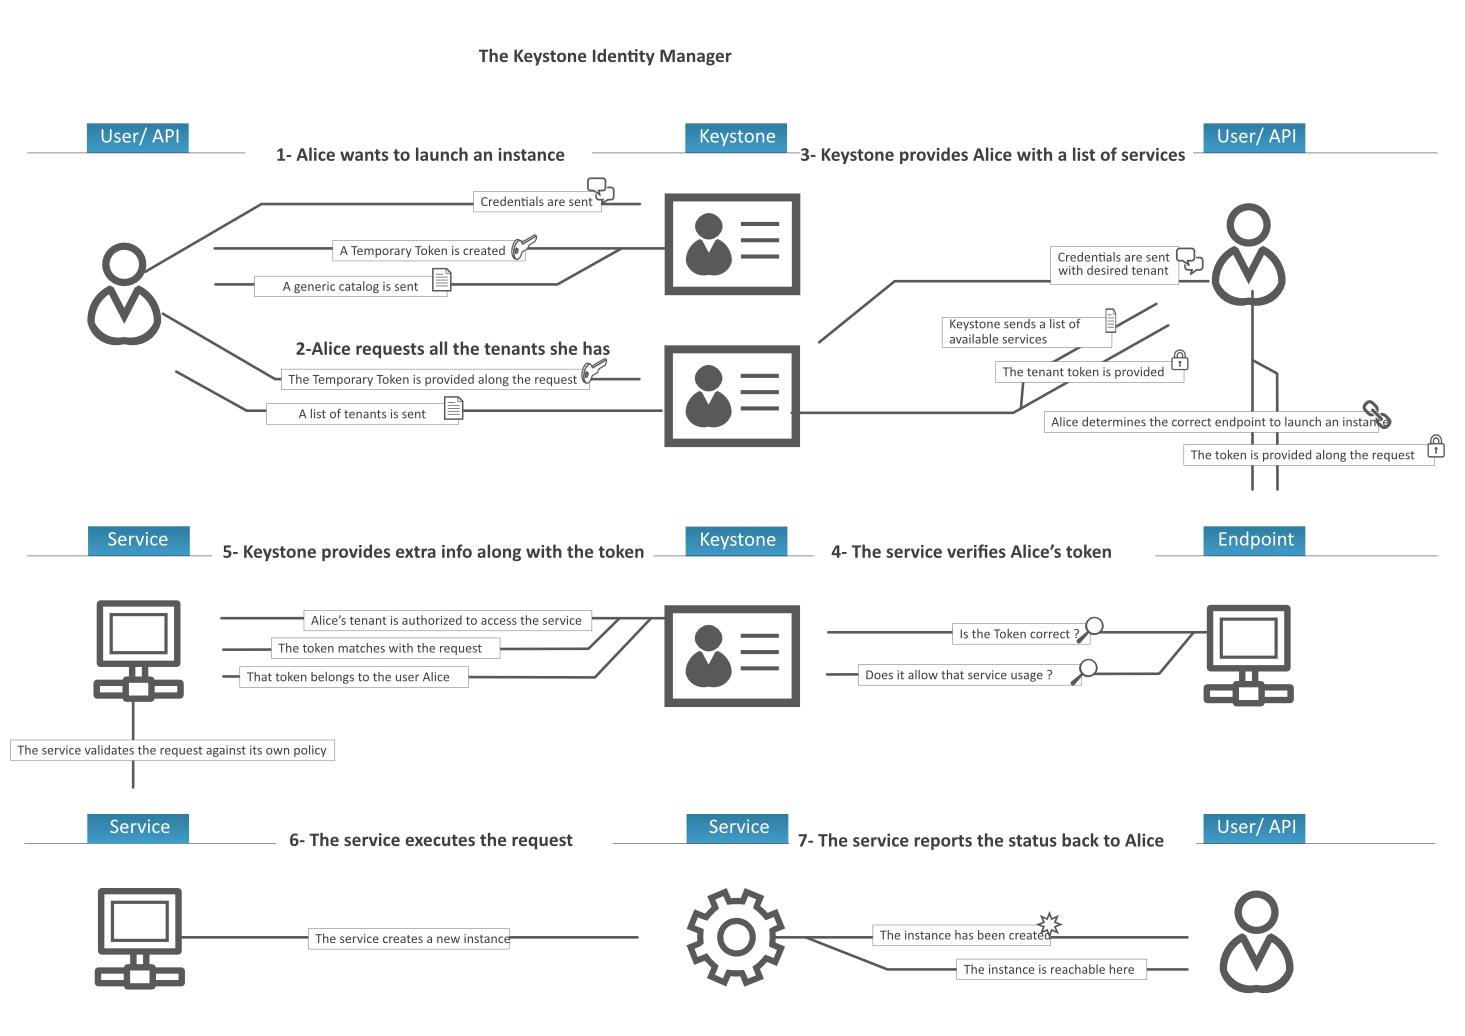
\includegraphics[scale=0.65, angle=90]{figures/keystone.png}
% 	\caption{Identity Service process flow}
% 	\label{fig:openstack_keystone}
% \end{figure} %%% [ref] http://docs.openstack.org/icehouse/install-guide/install/apt/content/keystone-concepts.html

\subsection{Horizon}
Horizon provides a modern web interface (an example is shown in Figure \ref{fig:dashboard}) that lets users and administrators interact with OpenStack services easily, instead of executing commands through a terminal. 
However, Horizon cannot completely replace the command line tool. For example, the web interface only proposes to choose the availability zone (i.e. a region in which a group of machines is located) when launching a virtual machine, but the command line tool lets you specify the host in the chosen availability zone.
The command line tool is particularily useful for the cloud administrator.

Once logged into the dashboard, users can launch instances and use them directly from a web browser via Virtual Network Computing (VNC) service configured during the installation of OpenStack.




%%--------------- section
\section{Setup}
\label{section_setup}
For our experiments, the ninth version of OpenStack, named \textit{Icehouse}\footnote{\url{https://www.openstack.org/software/icehouse/}} and released in April 2014, was installed and configured on three physical machines:

{
\singlespacing
\begin{itemize}
	\item{\texttt{controller} which acts as a controller node}
	\item{\texttt{compute1} which acts as a compute node}
	\item{\texttt{compute2} which acts as a compute node and a block storage node}
\end{itemize}
}

The installation of OpenStack was performed by following the OpenStack documentation \cite{osinstall}, that provides a step-by-step installation instructions.


\paragraph{Naming convention}\mbox{}\\
Each virtual machine created on the \texttt{compute1} node is called \texttt{vm1}, and each one created on the \texttt{compute2} node is called \texttt{vm2}. 
So, when \texttt{vm1} appear, it should be understand as \textit{the virtual machine hosted on \texttt{compute1}}.
If a virtual machine has a volume attached to it, \texttt{bs} (for Block Storage) will be attached to its name, becoming \texttt{vm1bs} for example. 
So, when \texttt{vm1bs} appear, it should be understand as \textit{the virtual machine hosted on \texttt{compute1} and with a volume attached to it}.
This convention is followed in the rest of this report.


%%--------------- subsubsection
\subsection{Machines}
This section describes the hardware used for the experiments.
In total, OpenStack services were installed on three machines.


\paragraph{Physical machines}\mbox{}\\
The three physical machines mentioned in Section \ref{section_setup} are HP Compaq Elite 8300 SFF with a 64-bit architecture. 
Each machine has an i7 3.4GHz Intel CPU, 16GB of RAM ($4\times4$GB DIMM DDR3 Synchronous 1600MHz) and a Western Digital HDD of 500GB. 
In the case of \texttt{compute2}, a partition of 100GB (93GB after partitioning with \textit{GParted}\footnote{Graphical editor for managing disk partitions (\url{http://gparted.org})}) was created in order to reserve space for the Block Storage service of OpenStack instead of a full disk recommended by the OpenStack documentation. 
Physical and logical volumes were created with the Logical Volume Manager (LVM) on the partition.
The machines are running Ubuntu 14.04 LTS 64-bit operating system. 
To create and run virtual machines, the open source hypervisor Kernel-based Virtual Machine (KVM) is used by the Compute Service. Each machine had one network interface card, instead of two interface cards recommended by the OpenStack documentation.


\paragraph{Virtual machines}\mbox{}\\
% The virtual machines are created on \texttt{compute1} and \texttt{compute2} nodes only are running a cloud image\footnote{Ubuntu cloud images can be found here: \url{https://cloud-images.ubuntu.com}} of Ubuntu Server 14.04 LTS prepared to run on cloud platforms like OpenStack. 
% A new flavor called \textit{physical} has been created and the flavor \textit{large} has been modified accordingly.\rp{tell why you need to create and modify flavors.}
% The updated list of flavors is now represented on Table \ref{table:flavors_list_2}. 
% For the experiments, only \textit{large} and \textit{physical} flavors were used. 
% With the \textit{physical} flavor, we try to have similar characteristics to a physical machine in order to compare them. 
% In this context, only one virtual machine with \textit{physical} flavor will be running at a time. 
% With the \textit{large} flavor, we try to have half of characteristics of a physical machine in order to have enough resources to run two virtual machines at the same time to benchmark application isolation.
The virtual machines are created on \texttt{compute1} and \texttt{compute2} nodes only are running a cloud image\footnote{Ubuntu cloud images can be found here: \url{https://cloud-images.ubuntu.com}} of Ubuntu Server 14.04 LTS prepared to run on cloud platforms like OpenStack. 

As the goal of this bachelor work is to evaluate the performance of OpenStack and compare it to the performance of the physical machines, we need new flavors that will reflect the characteristics of the physical machines.
Thus, a flavor called \textit{physical} has been created with the following values: 7 VCPUs and 13 GB of RAM.
These values are willingly a bit lower to the one observed on physical machines (8 VCPUs and 16 GB of RAM).
Indeed, as we want the virtual machine to use the same resources of a physical machine, the values of VCPUs and RAM should be lower in order for the instance to fit on one (which has already some resources used by running processes) without degrading the instance performance.
So, the \textit{physical} flavor is supposed to represent a (virtual) machine as powerful as a physical machine.

The \textit{m1.large} flavor (or simply \textit{large} flavor) is also relevant for the experiment as it represents half the power of a physical machine, so we can see how the number of VCPUs and the size of RAM can influence the performance results. 
It will also be useful to run two virtual machines at the same time to test isolation.
The disk size of this flavor has been updated to 30 GB to match the one set for the \textit{physical} flavor. 
The updated list of flavors is now represented on Table \ref{table:flavors_list_2}. 
Only \textit{large} and \textit{physical} flavors will be used to the experiment.

\begin{table}[h]
	\centering
	\begin{tabular}{|l|l|l|l|}
		\hline
		\textbf{Flavor} & \textbf{\# of VCPUs} & \textbf{Disk size (GB)} & \textbf{RAM size (MB)}\\
		\hline
		m1.tiny & 1 & 1 & 512 \\
		m1.small & 1 & 20 & 2048 \\
		m1.medium & 2 & 40 & 4096 \\
		m1.large & 4 & 30 & 8192 \\
		physical & 7 & 30 & 13312 \\
		m1.xlarge & 8 & 160 & 16384 \\
		\hline
	\end{tabular}
	\caption{Flavors}
	\label{table:flavors_list_2}
\end{table}



%%--------------- subsubsection
\subsection{OpenStack services} % TODO: or Components installation (?)
In this section, we briefly explain which OpenStack services are installed on what physical machines and their purposes.
The repartition of the different components is shown in Figure \ref{fig:os_arch}.

\begin{figure}[h]
	\centering
	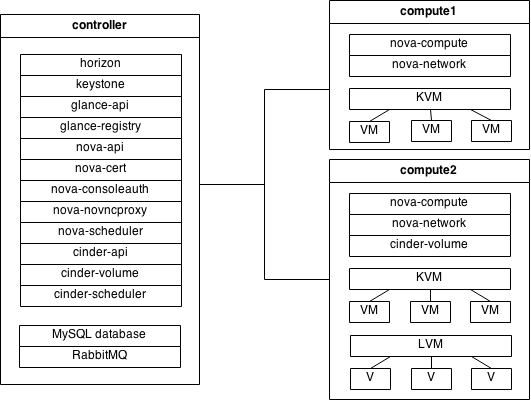
\includegraphics[scale=0.6]{figures/os_arch.png}
	\caption{Our OpenStack architecture}
	\label{fig:os_arch}
\end{figure}

The controller node is the heart of our OpenStack architecture, and thus all the different service APIs (Application Programming Interface) are installed on it. 
Keystone manages user accounts, and thus OpenStack services, as a new user is created for each service. 
Each request made by a service is handled by Keystone first: the service must authenticate against Keystone.
If this succeeds, then permissions are also checked, and if the permissions are sufficient, the request is accepted and further actions can be carried out by the service. 
Glance (\textit{glance-api} and \textit{glance-registry}) are also installed on the controller node. 
This means that all actions regarding OS images (creation, edition, deletion) are handled by the controller node.
Moreover all the different OS images are stored on it.
A web interface makes OpenStack easier to use, and for that Horizon is also installed on the controller node.
%, letting one access OpenStack with the following link \url{http://diufpc117.unifr.ch/horizon}\footnote{Access restricted to unifr network}. 
An overview of the dashboard is shown in Figure \ref{fig:dashboard}. 
It offers access to each service installed and, as an administrator, it is possible to manage them. 
To create, edit or delete an instance, a volume or an image, the user have to access these services through the \textit{Project} tab.
%
\begin{figure}[h]
	\centering
	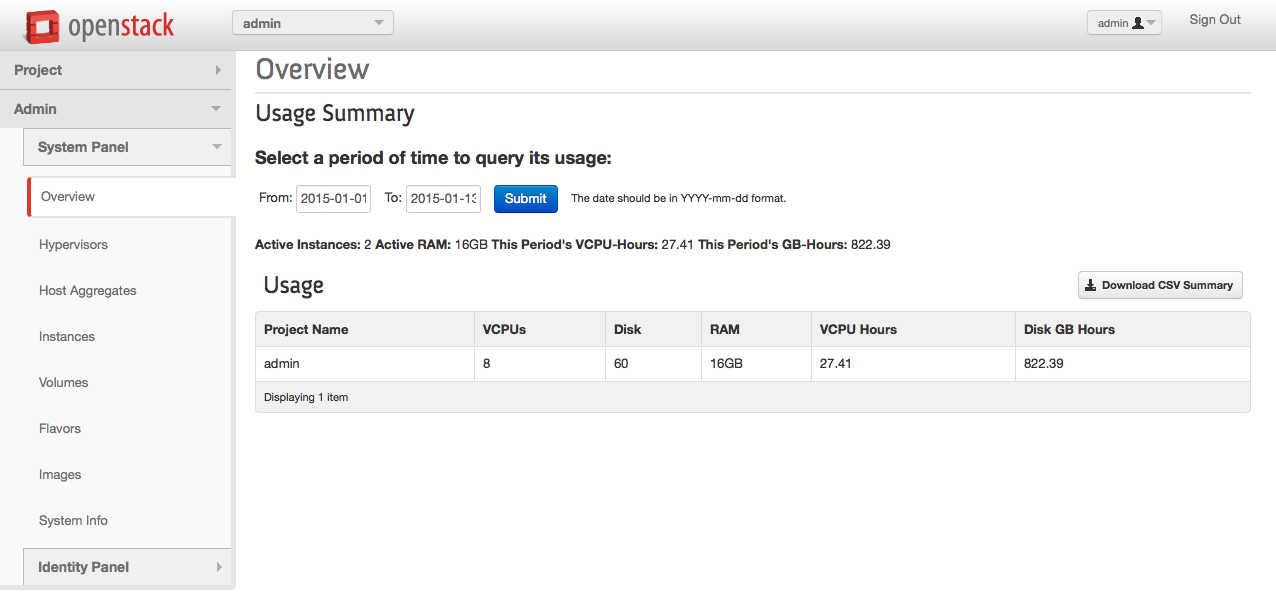
\includegraphics[scale=0.36]{figures/dashboard.png}
	\caption{Dashboard overview}
	\label{fig:dashboard}
\end{figure}
%
%TODO: nova -> describe each service?
In order to be able to create virtual machines, some components of Nova have to be installed on the controller node. These components exist for management purposes. 
Among them, we can mention \textit{nova-api}, \textit{nova-cert}, \textit{nova-consoleauth} and \textit{nova-novncproxy} for accessing an instance via VNC, and \textit{nova-scheduler} to determine on which physical machine an instance will run.
Likewise, \textit{cinder-api}, \textit{cinder-volume} and \textit{cinder-scheduler} components of the Cinder service are installed on the controller node for management purpose.
As each OpenStack service needs to store some information, a database is necessary. 
For this a \textit{MySQL}\footnote{\url{http://www.mysql.com}} database is installed and configured on the controller node. 
On any additional node (in our case, on \texttt{compute1} and \texttt{compute2}), only a MySQL client is installed to access the database hosted on the controller node.
%TODO: messaging system?


Compared to the controller node, \texttt{compute1} and \texttt{compute2} are less complex and do not need to run as many services as the controller.
For \texttt{compute1}, as its role is to create and host the virtual machines, two components of the Nova project are needed: \textit{nova-compute} and \textit{nova-network}. The first one is responsible for creating and terminating virtual machines. The second one is responsible for managing the network (bridging, updating iptables rules) for the virtual machines.

Finally, \texttt{compute2} has the same set of components as \texttt{compute1} regarding the Nova project. 
As this node also needs to take care of the creation and deletion of volumes, the \textit{cinder-volume} component of the Cinder service is installed on the node. 


